\chapter{Конструкторский раздел}
\label{ch:design}

\section{Выбор языка программирования}
\label{sec:language}
Для разработки приложений под Android используют, в основном, три языка программирования: Kotlin, Java и C++.

Kotlin стоит на первом месте не с проста.
В 2017 году компания Google объявила Kotlin новым официальным языком для Android и на то есть причины.
Java очень медленно развивалась, новые версии выходили с периодичностью раз в два-три года и новый функционал добавлялся крайне осторожно.
Например, в Java нет атрибутов класса, которые есть во многих современных языках, и приходится писать слишком много однотипного кода (геттеров и сеттеров) для тривиальной задачи "--- хранение внутреннего состояния объекта.

Еще одной большой проблемой Java является отсутствие null-безопасности.
То есть никогда нельзя быть уверенным, что в определенном месте кода объект не является null и есть вероятность получить NullPointerException в самом неожиданном месте.

Даже сейчас, когда Oracle внесла изменения в цикл релизов Java и выпускает их каждые полгода, это не спасёт Java для Android.
Причина тому "--- обратная совместимость приложений со старыми версиями Android API\@.
Например, поддержка Java 7 была добавлена в Android 4.4 (API 19, 2013 год), и эта версия считается стандартной целевой версией для широкой аудитории, так как на этой версии всё еще работает около 10\% устройств.
На более старых версиях суммарно работает меньше пяти процентов, поэтому именно эта версия позволяет достигнуть покрытия аудитории 95\%.
Поддержка Java 8 была добавлена только в Android N (API 24, 2016 год), но эта версия еще не скоро станет целевой, и трудно представить когда, при таких темпах обновления целевой версии, разработчики смогут использовать функции недавно вышедшей Java 10 или Java 11, которая выйдет через полгода.

Разработчикам на Android требовался современный, обновляющийся и простой язык, но при этом, чтобы можно было использовать существующие библиотеки, написанные на Java.
Сейчас существует много JVM языков, которые в той или иной мере совместимы с Java, но ни один из них, кроме Kotlin, не обрёл широкой популярности.
Scala "--- слишком сложна в освоении.
Groovy "--- допускает слишком много вольностей (даже самую простую задачу, например, объявление метода, можно решить несколькими способами), а динамическое выведение типов приводит к ошибкам во время выполнения.
И, что немаловажно, для этих языков нет хорошей IDE, которая бы поддерживала все их функции.
Kotlin же постарался вобрать в себя все положительные стороны каждого из языков, но и добавить своего и полностью исключить неоднозначности.
Тут есть удобные функциональные и nullable типы, как в Groovy, data-классы как в Scala, extension-функции и перегрузка операторов, как в C\# и т.д.
Kotlin разработан компанией JetBrains, которая занимается разработкой IntelliJ IDEA и поэтому проблем с поддержкой в IDE у него нет~\cite{kotlin:features}.

Например, чтобы объявить простой класс с несколькими внутренними состояниями и параметрами конструктора по умолчанию в Java потребуется такой код:\\

\begingroup
\javafile{inc/src/Student.java}
\captionof{listing}{Пример data-класса на Java\label{lst:studentJava}}
\endgroup

В Kotlin же для того чтобы выполнить ту же самую задачу потребуется гораздо меньше кода:

\begin{listing}[H]
  \kotlinfile{inc/src/Student.kt}
  \caption{Пример data-класса на Kotlin}
  \label{lst:studentKt}
\end{listing}

Вот пример null-безопасного кода на Kotlin:

\begin{listing}[H]
  \kotlinfile{inc/src/null.kt}
  \caption{Пример null-безопасности на Kotlin}
  \label{lst:nullKt}
\end{listing}

Kotlin очень быстро развивается и, в отличие от Java, для того чтобы использовать новую версию, достаточно лишь её подключить.
Kotlin полностью совместим с Java, а значит с ним можно использовать все библиотеки, написанные на Java, коих для Android очень много.

Среди языков разработки был упомянут еще C++.
Его используют только в специфических случаях, когда надо написать высокопроизводительный код.
Обычно это работа с графикой, звуком и т.д.
Минусом является то, что на С++ нельзя напрямую работать с Android SDK и нельзя использовать библиотеки, написанные на Java.

\begin{table}
  \caption{Сравнение языков программирования для Android}
  \label{tab:langs}
  \begin{tabular}{|P{0.4\textwidth}|c|c|c|}
    \hline
    Критерий & Kotlin~\cite{kotlin:features} & Java~\cite{java:main}& C++~\cite{cpp:main}\\
    \hline
    Прямая работа с Android SDK                       & $+$    & $+$  & $-$ \\
    \hline
    Наличие большого количества библиотек под Android & $+$    & $+$  & $-$ \\
    \hline
    Возможность управления памятью напрямую           & $-$    & $-$  & $+$ \\
    \hline
    Простой синтаксис                                 & $+$    & $-$  & $-$ \\
    \hline
    Data-классы, null-безопасность                    & $+$    & $-$  & $-$ \\
    \hline
  \end{tabular}
  \caption*{
    \small
    \raggedright
    \hspace{15mm}$+$ -- указанная возможность присутствует\\
    \hspace{15mm}$-$ -- указанная возможность отсутствует
  }
\end{table}

По итогам сравнения этих трёх языков программирования была составлена таблица~\ref{tab:langs}.
Был выбран язык Kotlin, как видно из таблицы, он имеет преимущество над остальными языками.


\section{Выбор среды разработки}
\label{sec:ide}
Были рассмотрены три среды программирования: Eclipse, Android Studio и IntelliJ IDEA\@.

\subsection{Eclipse}
\label{subsec:eclipse}
Свободная IDE для разработки модульных кросплатформенных приложений.
В стандартный пакет Eclipse не входят инструменты для создания Android приложений, но их можно добавить путём установки плагина.
Тем же путём можно добавить поддержку Kotlin.
Для Eclipse есть плагины для работы с Git, Gradle и прочими инструментами, полезными при разработке приложений.

\begin{figure}[ht]
  \centering
  \includegraphics[width=\textwidth]{inc/img/oxygen_darktheme_linux.jpg}
  \caption{Интерфейс Eclipse Oxygen}
  \label{fig:eclipse}
\end{figure}

Плюсом можно считать большое количество плагинов, возможность быстро и просто подключать новые языки, фреймворки и т.д.
Плагин для работы c Git репозиториями обладает большим количество функции и удобен в использовании.
Из минусов "--- Eclipse не понимает контекст.
Вернее понимает не так хорошо как IntelliJ IDEA или Android Studio.
Это проявляется, например, в подсказках при написании кода.
Eclipse просто подсказывает наиболее часто используемый вариант метода, поля и тому подобное, не глядя на контекст и зачастую это неудобно.
Редактор экранных форм не очень удобен~\cite{eclipse:oxygen}.

\subsection{IntelliJ IDEA}
\label{subsec:idea}
Это интегрированная среда разработки от компании JetBrains.
Её отличительными чертами являются: понимание контекста, наличие большого количества автоматических шаблонов рефакторинга, инспекции кода (инструменты анализа качества кода).

\begin{figure}[ht]
  \centering
  \includegraphics[width=\textwidth]{inc/img/idea_screenshot.png}
  \caption{Интерфейс IntelliJ IDEA 2018}
  \label{fig:idea}
\end{figure}

Есть две редакции: Community, с открытым исходным кодом и Ultimate, включающая все возможности редакции Community и дополнительные функции.
Бесплатная версия предлагает следующие возможности:
\Abbrev{VCS}{version control system "--- система контроля версий}
\begin{itemize}
  \item светлая и тёмная тема оформления;
  \item умное автодополнение, анализ качества кода, рефакторинги и форматирование кода "на лету" для Java и Kotlin;
  \item набор инструментов для разработки приложений под Android;
  \item отличная интеграция с VCS, с поддержкой таких полезных функций как частичные коммиты и сохранение контекста (открытых файлов, пакетов) для каждой ветки;
  \item интеграция с системами автоматической сборки: Gradle, Maven, Ant и другими;
  \item инструменты тестирования, с поддержкой множества библиотек и инструментов, таких как JUnit, Espresso, Spek, JaCoCo и др.
\end{itemize}

IDEA лучше всех других сред разработки поддерживает Kotlin потому как Kotlin тоже написан компанией JetBrains и все его новые функции тут же добавляются в IDE\@.

В Ultimate версии добавляется множество функций, но из наиболее полезных при разработке мобильных приложений можно отметить:
\begin{itemize}
  \item инструмент работы с базами данных и SQL файлами, удобный редактор схем БД, клиент и интеграция консоли для выполнения запросов в базу данных;
  \item поиск дубликатов кода;
  \item построение диаграмм классов и зависимостей.
\end{itemize}

Эта версия платная, но компания JetBrains предоставляет бесплатную лицензию для студентов и преподавателей~\cite{jetbrains:idea}.

\begin{figure}[ht]
  \centering
  \includegraphics[width=\textwidth]{inc/img/android_studio.jpg}
  \caption{Интерфейс Android Studio 3.0}
  \label{fig:as}
\end{figure}

\subsection{Android Studio}
\label{subsec:as}
Android Studio "--- это официальная интегрированная среда разработки для Android, на базе IntelliJ IDEA Community.
Она обладает всеми преимуществами и возможностями IntelliJ IDEA и добавляет следующие инструменты для написания Android-приложений:
\Abbrev{NDK}{native development kit}
\begin{itemize}
  \item эмулятор Android;
  \item шаблоны часто используемого при разработке приложений кода;
  \item поддержка С++ и NDK;
  \item редактор экранных форм;
  \item анализатор APK;
  \item профилировщик и инструменты отладки;
  \item возможность применения измененного кода без переустановки приложения (Instant Run)~\cite{android:as}.
\end{itemize}

В настоящее время, Android Studio основывается на IntelliJ IDEA 2017.3.3, а значит не включает в себя новых функций, доступных в IDEA 2018.
Это и есть основная проблема Android Studio.
Изменения Android Studio и IntelliJ IDEA сливаются друг в друга перекрёстно, то есть команда Android отвечает за доработку инструментов Android-разработки, а JetBrains за улучшение самой IDE\@.
IDEA часто обновляется и функционал из Android Studio сливают в неё быстрее, чем функционал новых версий IDEA в Android Studio.

\begin{table}
  \caption{Сравнение сред разработки для Android}
  \label{tab:ide}
  \begin{tabular}{|P{0.3\textwidth}|c|c|c|}
    \hline
    Критерий & Eclipse~\cite{eclipse:oxygen} & Android Studio~\cite{android:as}& IntelliJ IDEA~\cite{jetbrains:idea}\\
    \hline
    Поддержка Kotlin                   & $\pm$ & $+$ & $+$ \\
    \hline
    Инструменты для Android-разработки & $\pm$ & $+$ & $+$ \\
    \hline
    Понимание контекста                & $-$   & $+$ & $+$ \\
    \hline
    Частые обновления                  & $+$   & $-$ & $+$ \\
    \hline
    Инструменты для работы с БД        & $-$   & $-$ & $+$ \\
    \hline
  \end{tabular}
  \caption*{
  \small
  \raggedright
  \hspace{3mm}$+$ -- указанная возможность присутствует\\
  \hspace{3mm}$\pm$ -- указанная возможность может быть добавлена при помощи плагина\\
  \hspace{3mm}$-$ -- указанная возможность отсутствует
  }
\end{table}

По результатам проведенного обзора сред разработки составлена таблица~\ref{tab:ide}.
Выбрана IntelliJ IDEA, в силу того, что она содержит все возможности Android Studio, чаще обновляется и можно использовать возможности Ultimate версии.

\section{Выбор целевой версии Android API}
\label{sec:platform}

На официальном портале Android разработчиков размещена статистика, отображающая количество устройств, работающих под той или иной версией Android~\cite{android:distrib}.
По этим данным составлена таблица~\ref{tab:api}, на основе которой построена круговая диаграмма (рис.~\ref{fig:api}), наглядно показывающая долю устройств для каждой версии Android.

\begin{table}
  \caption{Доля устройств для каждой версии Android API}
  \label{tab:api}
  \begin{tabular}{|L|c|c|c|}
    \hline
    Версия       & Название                    & API & Доля устройств \\
    \hline
    2.3.3--2.3.7 & Gingerbread                 & 10  & 0.3\%          \\
    \hline
    4.0.3--4.0.4 & Ice Cream Sandwich          & 15  & 0.4\%          \\
    \hline
    4.1.x        & \multirow{3}{*}{Jelly Bean} & 16  & 1.5\%          \\
    \cline{1-1}\cline{3-4}
    4.2.x        &                             & 17  & 2.2\%          \\
    \cline{1-1}\cline{3-4}
    4.3          &                             & 18  & 0.6\%          \\
    \hline
    4.4          & Kit Kat                     & 19  & 10.3\%         \\
    \hline
    5.0          & \multirow{2}{*}{Lollipop}   & 21  & 4.8\%          \\
    \cline{1-1}\cline{3-4}
    5.1          &                             & 22  & 17.6\%         \\
    \hline
    6.0          & Marshmallow                 & 23  & 25.5\%         \\
    \hline
    7.0          & \multirow{2}{*}{Nougat}     & 24  & 22.9\%         \\
    \cline{1-1}\cline{3-4}
    7.1          &                             & 25  & 8.2\%          \\
    \hline
    8.0          & \multirow{2}{*}{Oreo}       & 26  & 4.9\%          \\
    \cline{1-1}\cline{3-4}
    8.1          &                             & 27  & 0.8\%          \\
    \hline
  \end{tabular}
  \caption*{
    \small
    \raggedright
    \hspace{30mm}Данные, собранные за неделю 1--7 мая 2018 года\\
    \hspace{30mm}Версии с долей устройств меньше 0.1\% не показаны
  }
\end{table}

\begin{figure}[ht]
  \centering
  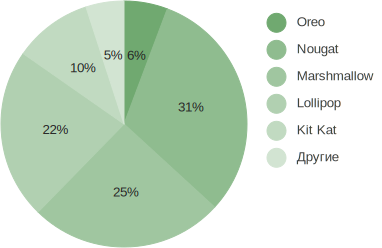
\includegraphics[width=.6\textwidth]{inc/svg/api_versions}
  \caption{Доля устройств для каждой версии Android}
  \label{fig:api}
\end{figure}

Android API обладает свойством обратно совместимости, а значит, приложение, написанное для старой версии API, будет работать на любой версии новее.
Например, приложение с целевой версией API 19 будет работать на API 27.
Исходя их этого можно посчитать, что целевая версия 19 даст 95\% покрытие устройств, 21 "--- 84.7\%, а 24 "--- всего 36.8\%.
В России эти показатели немного ниже, потому что доля устройств, с Android старее 4.4, выше, чем по миру~\cite{statcounter:api}.

\Abbrev{SVG}{scalable vector graphics "--- масштабируемая векторная графика}
Версии 19, 21 и 24 выбраны не случайно.
Версия 19 сейчас чаще всего используют как целевую, т.к. она обеспечивает 95\% покрытия устройств (в России 92.2\%).
Версия 21 тоже часто является целевой, потому что в ней был добавлен Material Design и поддержка SVG, что позволяет добиться одинакового вида приложения на всех устройствах.
В версии 24 была обновлена Java до 8 версии и добавлены функции, улучшающие безопасность: хранилища ключей, запрос разрешений в реальном времени и т.д.

\todo{Добавить таблицу сравнения целевых API}

\section{Выбор стека технологий}
\label{sec:stack}

\section{Архитектура и алгоритм работы МП СУПС}
\label{sec:architecture}

\section{Разработка пользовательского интерфейса}
\label{sec:gui}

\conclusions
\label{sec:designConclusions}
